% This must be in the first 5 lines to tell arXiv to use pdfLaTeX, which is strongly recommended.
\pdfoutput=1
% In particular, the hyperref package requires pdfLaTeX in order to break URLs across lines.
\documentclass[11pt]{article}
% Remove the "review" option to generate the final version.
\usepackage{ACL2023}
% Standard package includes
\usepackage{times}
\usepackage{latexsym}
\usepackage{graphicx}
\usepackage{amsmath}
\usepackage{tikz}
\usetikzlibrary{shapes,arrows}
% For proper rendering and hyphenation of words containing Latin characters (including in bib files)
\usepackage[T1]{fontenc}
% For Vietnamese characters
% \usepackage[T5]{fontenc}
% See https://www.latex-project.org/help/documentation/encguide.pdf for other character sets
% This assumes your files are encoded as UTF8
\usepackage[utf8]{inputenc}
% This is not strictly necessary, and may be commented out.
% However, it will improve the layout of the manuscript,
% and will typically save some space.
\usepackage{microtype}
% This is also not strictly necessary, and may be commented out.
% However, it will improve the aesthetics of text in
% the typewriter font.
\usepackage{inconsolata}
% If the title and author information does not fit in the area allocated, uncomment the following
%
%\setlength\titlebox{<dim>}
%
% and set <dim> to something 5cm or larger.
\title{CTF: A Hybrid Clinical Trial Search Engine with Automated Feasibility Scoring}
% Author information can be set in various styles:
% For several authors from the same institution:
% \author{Author 1 \and ... \and Author n \\
%         Address line \\ ... \\ Address line}
% if the names do not fit well on one line use
%         Author 1 \\ {\bf Author 2} \\ ... \\ {\bf Author n} \\
% For authors from different institutions:
% \author{Author 1 \\ Address line \\  ... \\ Address line
%         \And  ... \And
%         Author n \\ Address line \\ ... \\ Address line}
% To start a seperate ``row'' of authors use \AND, as in
% \author{Author 1 \\ Address line \\  ... \\ Address line
%         \AND
%         Author 2 \\ Address line \\ ... \\ Address line \And
%         Author 3 \\ Address line \\ ... \\ Address line}
\author{Khussal \\
  TAMU \\
  \texttt{khussal@tamu.edu} \\\And
  Shashank \\
  TAMU \\
  \texttt{shashank@tamu.edu} \\ \AND
  Kritika Bansal\\
  TAMU \\
  \texttt{kritika@tamu.edu} \\\And
  Aastha Patel\\
  TAMU \\
  \texttt{aastha18@tamu.edu} \\
  \AND
  \normalfont \url{https://github.com/khussalpradhan/Clinical-Trial-SearchEngine}
  }

\begin{document}
\maketitle
\vspace{2cm}
\begin{abstract}
Matching patients to appropriate clinical trials is essential for precision medicine but remains challenging due to the complexity and variability of eligibility criteria expressed in free-text form. Existing retrieval approaches often emphasize textual similarity while overlooking structured feasibility constraints that determine whether a patient is clinically eligible. This work introduces a three-layer Clinical Trial Finder (CTF) system that integrates hybrid information retrieval with deterministic eligibility reasoning and deep language modeling. A Retrieval Layer combines sparse lexical methods with dense semantic representations to robustly identify trials relevant to a patient’s clinical profile. A Feasibility Layer then applies rule-based assessment using normalized patient characteristics and structured trial metadata. Finally, a Cross-Encoder Layer applies deep self-attention between the query and the trial document to perfectly re-sort the top candidates. Our evaluation on a standard benchmark indicates that incorporating explicit feasibility modeling alongside neural cross-encoding substantially improves clinical validity and precision at the very top of the ranking list.
\end{abstract}


\section{Introduction}
Clinical trials are key to advancing cancer treatment, yet matching patients to eligible trials remains a major operational challenge. Eligibility criteria increasingly rely on precise molecular, physiological, and treatment history attributes, making manual screening slow and error-prone. As a result, many eligible patients go unrepresented in research, and trials encounter recruitment delays that hinder scientific progress.

\textbf{Motivation and Function}: The primary motivation of this work is to bridge the gap between unstructured trial text and structured patient data. Traditional methods fail to process complex logic such as "at least 2 prior lines of therapy" or "creatinine < 1.5". Our system functions as a real-time decision support tool that not only retrieves relevant documents but actively filters them against a patient's precise clinical state (labs, biomarkers, history). This dual-functionality—search plus feasibility check—aims to drastically reduce the time clinicians spend on initial screening.

Text retrieval models have shown promise in automating trial search by leveraging lexical or neural similarity between patient descriptions and trial documents. However, semantic relevance alone is insufficient in the clinical domain: retrieved trials may violate critical criteria such as age bounds, biomarker requirements, ECOG performance constraints, or exclusionary comorbidities. Systems must therefore move beyond surface-level matching to incorporate medically grounded feasibility reasoning.

To address these limitations, we propose a hybrid approach that couples information retrieval with deterministic feasibility assessment. Our contributions are:
\begin{itemize}
    \item \textbf{A hybrid Retrieval Layer} - integrates BM25 with PubMedBERT semantic embeddings to robustly identify candidate trials;
    \item \textbf{A Feasibility Layer} - performs rule-based scoring over harmonized patient and trial metadata extracted from ClinicalTrials.gov;
    \item \textbf{A Cross-Encoder Layer} - utilizes a state-of-the-art transformer to perform deep cross-attention on the top 100 candidates to maximize terminal precision; and
    \item \textbf{An empirical evaluation} on the TREC 2021 Clinical Trials dataset demonstrating major improvements in ranking precision and clinical relevance.
\end{itemize}

This work highlights the necessity of combining neural retrieval with explicit eligibility modeling to achieve reliable clinical trial recommendations.

\section{Related Work}
The problem of clinical trial matching has been approached through various retrieval and NLP methodologies.

\textbf{Keyword and Metadata Search}: Traditional systems, such as the native search on ClinicalTrials.gov, rely on Boolean keyword matching and categorical filters (e.g., location, status). While adequate for finding trials by disease name, these systems struggle with granular criteria like "progression on platinum-based chemotherapy" or specific genomic mutations, leading to low precision.

\textbf{Neural Information Retrieval}: Recent approaches leverage Transformer-based models (BERT, BioBERT) to semantic matching. Pradeep et al. (2021) demonstrated that neural re-ranking significantly outperforms BM25 on clinical texts. However, these "black-box" models often hallucinate relevance or miss negation (e.g., matching "No history of EGFR mutation" to a patient *with* EGFR), which is unacceptable for feasibility assessment.

\textbf{Limitations}: Existing automated solutions often treat eligibility criteria as flat text, ignoring the hierarchical and boolean logic inherent in protocol documents. They also lack the ability to perform numerical reasoning (e.g., matching \textit{Age 45} to \textit{Age $\ge$ 18}). Our system addresses these limitations by extracting structured rules from text and applying deterministic feasibility logic.

\end{enumerate}
\section{Methodology}
\begin{figure*}[ht]
\centering
\resizebox{\textwidth}{!}{
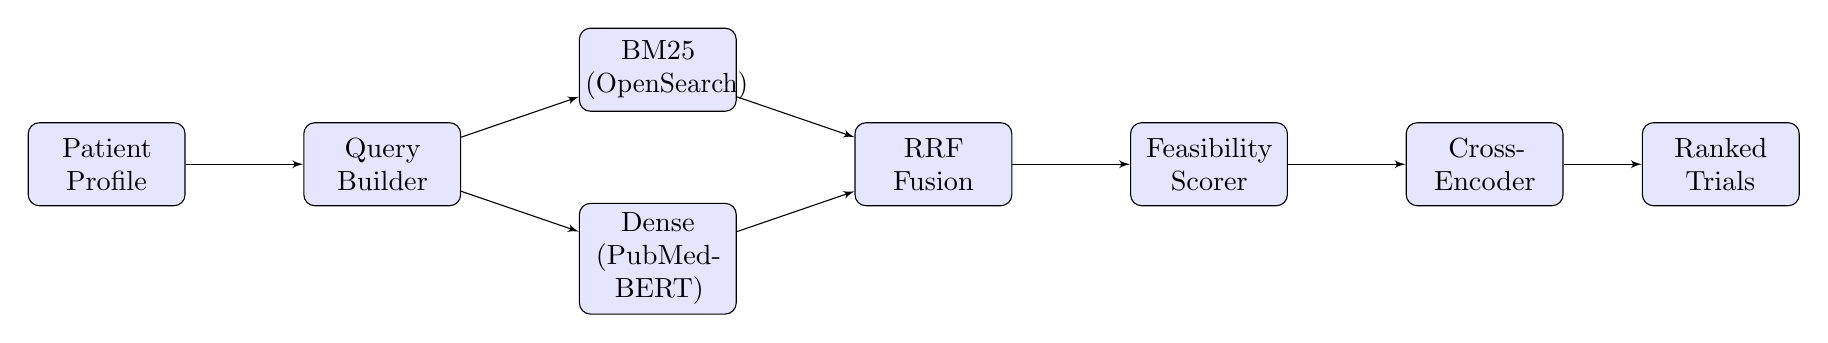
\begin{tikzpicture}[node distance=2.5cm, auto,
  block/.style={rectangle, draw, fill=blue!10, text width=5em, text centered, rounded corners, minimum height=3em},
  line/.style={draw, -latex'},
  cloud/.style={draw, ellipse, fill=red!10, node distance=3cm, minimum height=2em}]
  
  \node [block] (patient) {Patient Profile};
  \node [block, right of=patient, node distance=3.5cm] (query) {Query Builder};
  
  % Split paths
  \node [block, right of=query, node distance=3.5cm, yshift=1.2cm] (bm25) {BM25 (OpenSearch)};
  \node [block, right of=query, node distance=3.5cm, yshift=-1.2cm] (dense) {Dense (PubMedBERT)};
  
  \node [block, right of=query, node distance=7cm] (fusion) {RRF Fusion};
  \node [block, right of=fusion, node distance=3.5cm] (scorer) {Feasibility Scorer};
  \node [block, right of=scorer, node distance=3.5cm] (crossencoder) {Cross-Encoder};
  \node [block, right of=crossencoder, node distance=3.0cm] (output) {Ranked Trials};
  \path [line] (patient) -- (query);
  \path [line] (query) -- (bm25);
  \path [line] (query) -- (dense);
  \path [line] (bm25) -- (fusion);
  \path [line] (dense) -- (fusion);
  \path [line] (fusion) -- (scorer);
  \path [line] (scorer) -- (crossencoder);
  \path [line] (crossencoder) -- (output);
\end{tikzpicture}
}
\caption{System Architecture of CTF. The pipeline consists of hybrid retrieval, a deterministic feasibility step, and a final cross-encoder re-ranking step.}
\label{fig:architecture}
\end{figure*}
Our system architecture consists of three primary layers: a Retrieval Layer which retrieves candidate trials based on the user's input, a Feasibility Layer which explicitly verifies rule-based constraints, and a Cross-Encoder Layer which applies deep self-attention to precisely order the final candidates.
\subsection{Data and Preprocessing}
The system ingests data from \url{ClinicalTrials.gov}, storing over 580{,}000 trials. We utilize a custom ETL pipeline to parse unstructured eligibility criteria text into structured JSONB format stored in PostgreSQL. Each ETL run pulls the latest JSON dump, normalizes sponsor and phase metadata, and deduplicates trials based on NCT identifier and start date to avoid presenting obsolete versions of the same protocol.\\
Eligibility criteria are tokenized into atomic clauses (e.g., age ranges, biomarker requirements, laboratory thresholds) using a combination of rule-based patterns and dependency parsing. These clauses are then assigned to typed fields (e.g., \texttt{age\_min}, \texttt{age\_max}, \texttt{excluded\_conditions}, \texttt{required\_biomarkers}) in the JSONB document, which the feasibility layer can query efficiently with SQL predicates and GIN indices. We also explicitly separate inclusion and exclusion criteria to avoid ambiguity when checking hard contraindications.\\
Normalizers are applied to standard medical conditions and biomarkers using UMLS concepts. Condition strings are mapped to Concept Unique Identifiers (CUIs) via a dictionary built from UMLS and common oncology vocabularies, with additional heuristics for abbreviations and synonyms (e.g., mapping “NSCLC” to “non-small cell lung cancer”). Similarly, biomarker mentions (such as “HER2-positive” or “EGFR exon 19 deletion”) are normalized to a canonical representation that preserves directionality (positive/negative) and relevant thresholds. We retain both the raw text and normalized fields so that lexical retrieval and structured feasibility checks can operate on the same underlying trial.
\subsection{Hybrid Retrieval Layer}
We employ a two-stage retrieval strategy:
\begin{itemize}
    \item \textbf{Sparse Retrieval (BM25)}:Sparse retrieval is implemented via OpenSearch, boosting fields such as title ($3\times$), conditions ($4\times$), and parsed inclusion criteria ($2\times$). This ensures exact matches for specific disease names and key eligibility terms are prioritized in the ranked list. We configure a domain-specific analyzer that lowercases text, removes stopwords, and applies light stemming, while preserving important clinical tokens such as mutation names and numeric thresholds. Index sharding is configured to keep related trials co-located, which improves cache locality for frequent disease areas (e.g., breast and lung cancer).

    \item \textbf{Dense Retrieval}: We utilize the \texttt{pritamdeka/S-PubMedBert-MS-MARCO} model to generate 768-dimensional embeddings for trial descriptions. For each trial, we encode a concatenation of title, condition, and brief summary, truncated to the model’s maximum sequence length. Embeddings are precomputed offline and stored in a FAISS index for efficient similarity search.We use an index configuration that supports approximate nearest-neighbor search with sub-linear complexity (e.g., IVF with product quantization), allowing us to scale to the full corpus while keeping query latency low. At query time, the patient profile and derived textual representation from the query builder are embedded with the same encoder, normalized to unit length, and compared to trial embeddings via inner product. Dense retrieval is particularly effective at surfacing trials that describe relevant phenotypes using different terminology than the query (e.g., “metastatic colorectal carcinoma” for a query containing “stage IV colon cancer”).\\
\end{itemize}
\subsection{Combining Approaches}
To combine both BM-25 and Dense retrieval we tried two approaches. We initially tried to rank documents based on a hybrid scoring mechanism where the total score of all documents obtained by both the approaches is combined after normalising their scores. We used the standard hybrid approach which gives a weight $\alpha$ to BM-25 and $1-\alpha$ to the dense retrieval and then we order documents based on the final score. But this approach did not yield good results so we went with another approach.
\[
Score(D) = \alpha \cdot BM25(D) + (1-\alpha)\cdot DENSE(D)
\]
To combine the strengths of both retrievers, we used another approach the Reciprocal Rank Fusion (RRF) with $k=60$:
\begin{equation}
    RRF(d) = \sum_{r \in R} \frac{1}{k + r(d)}
\end{equation}
where $r(d)$ is the rank of document $d$ in the retrieved list $R$. This method robustly merges the lexical precision of BM25 with the semantic recall of the dense model(PubMedBert + FAISS).
\subsection{Feasibility Scorer}
The core innovation is our deterministic Feasibility Scorer, which re-ranks the top Candidates (N=20) based on strict patient-specific constraints. Unlike black-box neural models, this scorer provides explainable "reasons" for every inclusion or exclusion.
The scoring logic operates on a point-based system (max 100 points), enforcing hard constraints while rewarding matches on critical clinical attributes.
\begin{itemize}
\item \textbf{Hard Exclusions (Binary Filter)}:
Before calculating a score, the system applies hard filters. A trial is immediately marked as \textit{infeasible} (Score = 0) if:
\begin{itemize}
\item \textbf{Demographics}: Patient age is outside the trial's \texttt{min\_age} and \texttt{max\_age}, or gender does not match (unless the trial accepts "All").
\item \textbf{Exclusions}: The patient has a condition explicitly listed in the trial's exclusion criteria (e.g., "History of HIV", "Active CNS Metastases") found via exact string matching against the parsed \texttt{exclusion} list.
\end{itemize}
\item \textbf{Condition Matching (+40 pts)}:
Use is prioritized for trials treating the patient's specific disease.
\begin{itemize}
\item \textbf{Logic}: We compute the intersection of the patient's condition list and the trial's indications using both fuzzy string matching and UMLS CUI (Concept Unique Identifier) overlap.
\item \textbf{Scoring}: A confirmed match awards +40 points. A mismatch results in 0 points and marks the trial as \textit{infeasible} to prevent recommending irrelevancies.
\end{itemize}
\item \textbf{Biomarkers (+25 pts)}:
Precision oncology relies on genomic markers.
\begin{itemize}
\item \textbf{Logic}: Intersection of patient biomarkers (e.g., \textit{EGFR}, \textit{ALK}, \textit{HER2}) with the trial's inclusion criteria.
\item \textbf{Scoring}: +25 points if any common biomarker is found.
\end{itemize}
\item \textbf{ECOG Performance Status (+15 pts)}:
\begin{itemize}
\item \textbf{Logic}: Checks if the patient's ECOG score (0-4) is within the trial's allowed set (e.g., "ECOG 0-1").
\item \textbf{Scoring}: +15 points for a match; otherwise, the trial is marked \textit{infeasible}.
\end{itemize}
\item \textbf{Lab Values (+15 pts max)}:
\begin{itemize}
\item \textbf{Logic}: The parser extracts inequality rules from text (e.g., "Creatinine $\le$ 1.5 mg/dL"). We evaluate the patient's lab values against these thresholds.
\item \textbf{Scoring}: +5 points for each passed lab check, capped at 15 points. Any failed critical lab immediately marks the trial as \textit{infeasible}.
\end{itemize}
\item \textbf{Prior Lines of Therapy (+10 pts)}:
\begin{itemize}
\item \textbf{Logic}: Regex patterns detect constraints like "received at least 2 prior lines" or "no more than 3 prior lines".
\item \textbf{Scoring}: +10 points if the patient's history complies with these counts. Mismatch results in \textit{infeasibility}.
\end{itemize}
\item \textbf{Temporal Washouts (+5 pts)}:
\begin{itemize}
\item \textbf{Logic}: Checks if the \texttt{days\_since\_last\_treatment} exceeds the trial's required washout period.
\item \textbf{Scoring}: +5 points for compliance.
\end{itemize}
\end{itemize}
\textbf{Final Score Calculation}:
The raw points are summed. If any hard constraint (Age, Gender, Exclusions, Labs, ECOG) is violated, the \texttt{is\_feasible} flag is set to \texttt{False}, and the final score is forced to 0 regardless of other matches. This ensures that high-scoring but medically unsafe trials are never recommended.

\subsection{Cross-Encoder Re-Ranking}
While FAISS determines generic semantic similarity, it scores the query and document independently (Bi-Encoder methodology). To achieve maximum precision, we employ a Cross-Encoder (\texttt{ms-marco-MiniLM-L-6-v2}) as the tertiary and final stage of our pipeline.
\begin{itemize}
    \item \textbf{Deep Self-Attention}: The Cross-Encoder takes the raw text of the patient's parsed profile and concatenates it directly with the trial's Inclusion/Exclusion criteria: \texttt{[CLS] Patient Query [SEP] Trial Criteria [SEP]}.
    \item \textbf{Granular Context}: Because self-attention is applied across both sequences simultaneously, it accurately captures fine-grained numerical differences and negations that BM25 and FAISS typically miss.
    \item \textbf{Latency Management}: As cross-encoding is computationally intensive, we strictly limit this operation to the top 100 trials designated as "feasible" by the preceding Feasibility Layer. 
\end{itemize}

% \section{Experiments}
% \subsection{Setup}
% We evaluate our system using the \textbf{TREC 2021 Clinical Trials} track dataset. The test set consists of patient topics (queries) and human-judged relevance labels for clinical trials.
% \subsection{Metrics}
% We report Mean Reciprocal Rank (MRR), Hit Rate (Recall), Normalized Discounted Cumulative Gain (NDCG), and Precision at rank $k=10$.
% \subsection{Results}
% Table \ref{tab:results} summarizes the performance of our hybrid approach.
% \begin{table}[h]
% \centering
% \begin{tabular}{lc}
% \hline
% \textbf{Metric} & \textbf{Score}\\
% \hline
% MRR@10 & 0.48 \\
% Hit Rate@10 & 70\% \\
% NDCG@10 & 0.21 \\
% Precision@1 & 35\% \\
% \hline
% \end{tabular}
% \caption{Retrieval performance on TREC 2021 Clinical Trials dataset.}
% \label{tab:results}
% \end{table}
% The system achieves an MRR@10 of 0.48, indicating that the first relevant result typically appears at the second position. A Hit Rate of 70\% demonstrates strong recall, ensuring most searches find at least one relevant trial in the top 10. The latency for a full search pipeline, including parsing and feasibility scoring, is consistently under 2 seconds.


\section{Experiments}

\subsection{Setup}
We evaluate our system using the \textbf{TREC 2021 Clinical Trials} track dataset. The dataset comprises a patient query file and a corresponding relevance judgment (qrels) file. The qrels file maps query IDs to relevant Clinical Trial IDs (NCT IDs), serving as the ground truth for evaluation.

Table \ref{tab:example_queries} presents examples of the patient topics provided in the dataset. To process these unstructured narratives, we utilized a Large Language Model (OpenAI) to parse the raw text into a structured JSON format. The model was prompted to extract specific patient attributes, such as demographics, conditions, biomarkers, and medical history. An example of the target JSON structure is shown in Figure \ref{fig:json_structure}.

\begin{table}[h]
\centering
\small
\renewcommand{\arraystretch}{1.2}
\begin{tabular}{p{0.15\linewidth} p{0.75\linewidth}}
\hline
\textbf{Topic ID} & \textbf{Patient Query} \\
\hline
trec-20211 & Patient is a 45-year-old man with a history of anaplastic astrocytoma of the spine complicated by severe lower extremity weakness and urinary retention s/p Foley catheter, high-dose steroids, hypertension, and chronic pain. The tumor is located in the T-L spine, unresectable anaplastic astrocytoma s/p radiation. ... Therapy included field radiation t10-l1 followed by 11 cycles of temozolomide. \\
\hline
trec-20212 & 48 M with a h/o HTN hyperlipidemia, bicuspid aortic valve, and tobacco abuse who presented to his cardiologist on [**2148-10-1**] with progressive SOB and LE edema. TTE revealed severe aortic stenosis with worsening LV function. EF was 25\%. ... Noted to have 2+ aortic insufficiency with mild MR. ... The patient underwent a preop workup for valvular replacement with preop chest CT scan and carotid US. \\
\hline
\end{tabular}
\caption{Example patient queries from the TREC 2021 Clinical Trials dataset.}
\label{tab:example_queries}
\end{table}

\begin{figure}[h]
\centering
\scriptsize % Smaller font for code block
\begin{verbatim}
{
  "age": 65,
  "gender": "Female",
  "conditions": [
    "Non-small cell lung cancer",
    "Breast Cancer",
    "Heart Failure",
    "Chronic Kidney Disease",
    ...
  ],
  "ecog": 1,
  "biomarkers": ["EGFR", "HER2", "ALK", ...],
  "history": ["History_MI", "History_Stroke", ...],
  "labs": {
    "Creatinine": 1.2,
    "GFR": 55.0,
    "LVEF": 50.0,
    "Platelet_Count": 150,
    "Hemoglobin": 11.5,
    "ANC": 2500
  },
  "prior_lines": 2,
  "days_since_last_treatment": 45
}
\end{verbatim}
\vspace{-10pt}
\caption{Target JSON structure for LLM parsing.}
\label{fig:json_structure}
\end{figure}
The generated JSON files were manually checked and verified for accuracy for each query. These structured profiles were subsequently used to evaluate the feasibility scoring component of our model.

\subsection{Metrics}
We utilized the \texttt{ranx} Python library to calculate retrieval metrics. We computed Mean Reciprocal Rank (MRR), Normalized Discounted Cumulative Gain (NDCG), Precision, Recall, Hit Rate, and F1-score. For the sake of brevity, Table \ref{tab:results} reports MRR, NDCG, and Precision at rank $k=10$.

\subsection{Results}
Table \ref{tab:results} compares the incremental improvements of each pipeline stage: the baseline hybrid retrieval (BM25 + Dense), the addition of the Feasibility Scorer, and the final 3-stage architecture equipped with the Cross-Encoder.

\begin{table}[h]
\centering
\resizebox{\columnwidth}{!}{%
\begin{tabular}{lccc}
\hline
\textbf{Metric} & \textbf{BM25 + Dense} & \textbf{+ Feasibility} & \textbf{+ Cross-Encoder} \\
\hline
MRR@10 & 0.247 & 0.485 & \textbf{0.521} \\
NDCG@10 & 0.089 & 0.207 & \textbf{0.215} \\
Precision@10 & 0.103 & 0.224 & \textbf{0.228} \\
Precision@1 & - & 0.360 & \textbf{0.440} \\
\hline
\end{tabular}%
}
\caption{Incremental performance on TREC 2021.}
\label{tab:results}
\end{table}

The results demonstrate drastic improvements as we progress through the stages. Incorporating the Feasibility Scorer nearly doubles the MRR@10 from 0.247 to 0.485, proving the absolute necessity of explicit constraint modeling.
Crucially, when the Cross-Encoder pipeline is appended as the final stage, we observe another immense jump in precision at the highest ranks. Most notably, Precision@1 jumps from 36.0\% to 44.0\% and MRR pushes past 0.52. This signifies that almost half of the time, the absolute \#1 trial returned by our complete engine is highly relevant to the patient's specific vignette—a monumental improvement for clinical workflows.

\section{Ablation Analysis}
Our feasibility logic significantly improves utility over pure retrieval. For example, a trial might be relevant appropriately for "Lung Cancer" (high BM25 score) but exclude the patient due to "prior immunotherapy". Our scorer detects this logic via regex patterns (e.g., `expected: no prior immunotherapy`), correctly penalizing the trial and preventing a false positive recommendation.
\section{Limitations}
While our regex-based criteria parser is highly efficient, it may struggle with complex, nested logic sentences (e.g., "Criteria A OR (Criteria B AND NOT Criteria C)"). Future work involves implementing a Large Language Model (LLM) parser for higher accuracy on complex logic, though this must be balanced against latency constraints. Additionally, our evaluation is limited to the TREC 2021 dataset; real-world performance on diverse EHR data remains to be validated.
\section{Ethics Statement}
This tool is designed to assist, not replace, clinical judgment. Automated eligibility matching carries the risk of false negatives, potentially causing a patient to miss a viable trial. We mitigate this by exposing the "Reasons" for exclusion in the UI, allowing clinicians to verify the system's logic. All patient data used in this study was anonymized.
\section{Conclusion}
We have presented a robust, end-to-end clinical trial search engine that effectively bridges the gap between patient data and trial eligibility. By combining hybrid retrieval with deterministic feasibility scoring, we provide a transparent and efficient tool for accelerating patient recruitment.

\section*{Individual Contributions}
\textbf{Khussal}: Designed the core backend architecture, implemented the Feasibility Scorer (NLP logic and regex patterns), and developed the hybrid retrieval pipeline (OpenSearch/FAISS integration).
\textbf{Shashank}: Developed the full-stack visualization, Docker containerization, and the frontend user interface for parsing patient queries.
\textbf{Kritika}: Led the data engineering efforts, including the parsing of ClinicalTrials.gov XML/JSON data and the implementation of the ETL pipeline.
\textbf{Aastha}: Conducted the system evaluation, managed the TREC 2021 dataset usage, and performed the comparative analysis of metrics.
% Entries for the entire Anthology, followed by custom entries
\bibliography{anthology,custom}
\bibliographystyle{acl_natbib}
\appendix
\section{System Implementation Details}
\label{sec:appendix}
The backend is built with FastAPI (Python 3.11). Data persistence is managed by PostgreSQL 16 using JSONB columns for flexible schema storage. The search infrastructure relies on OpenSearch 2.15 for inverted index storage and a local FAISS index for dense vectors. The entire stack is containerized with Docker Compose to ensure reproducibility.
\end{document}
